\documentclass[a4paper,11pt, twocolumn]{article}
%\usepackage[T1]{fontenc} %for å bruke æøå
\usepackage[utf8]{inputenc}
\usepackage[T1]{fontenc}
\usepackage[norsk]{babel}
\usepackage{graphicx} %for å inkludere grafikk
\usepackage{verbatim} %for å inkludere filer med tegn LaTeX ikke liker
\usepackage{mathpazo}
\usepackage{mathtools}
\usepackage{csquotes}
\usepackage{tikz}
\usepackage{listings}
\usepackage{booktabs}
\usepackage{todonotes}
\usepackage[backend=biber]{biblatex}
\usepackage{caption} 
\usepackage{parboxx}
\hyphenpenalty=750
\captionsetup[table]{skip=10pt}

%\addbibresource{solceller.bib}

\lstset{language=Matlab, commentstyle=\textcolor[rgb]{0.00,0.50,0.00}, keepspaces=true, columns=flexible, basicstyle=\footnotesize, keywordstyle=\color{blue}, showstringspaces=false, inputencoding=ansinew}

\title{Rapport 3 FYS2150\\Solcellen}

\author{Eivind Brox}
\date{\today}

\begin{document}

\maketitle
\listoftodos
\begin{abstract}

\end{abstract}

\section{Introduksjon}
Energi er et viktig tema innenfor vitenskap, økonomi og politikk. Det diskuteres stadig hvilke kilder det skal satses på, og hvilke som bør fases ut til fordel for et mer menneskevennlig klima på jorden. 

I utgangspunktet er det bare tre kilder til energi som påvirker jorden. Solen er den som bidrar sterkest til energien mennesker nyttiggjør seg av idag. Geotermisk energi fra jorden indre prosesser utnyttes i mindre grad, og energi fra kosmisk stråling har lite potensial.

Solen varmer opp og skaper bevegelse i havene, den setter lufta i bevegelse og får planter til å vokse. Alt disse effektene kan brukes til å indirekte høste energi fra solen. Det kunne kanskje være interessant å høste energien mer direkte fra solen og kvitte seg med flere av mellomleddene?

Solceller lar oss gjøre nettopp dette. Mellomledd er fortsatt til stede, men energien er momentant tilgjengelig så lenge solen skinner. Utfordringer knyttet til solcelleteknologi dreier seg om å effektivisere produksjon og drift. I denne rapporten ser vi nettopp på solcellens virkemåte i forhold til hvordan cellene kobles sammen, hvilken last som bør brukes for å oppnå maksimal effekt og hvilke bølgelengder som gir størst effektivitet.   
\section{Teori}
\section{Eksperimentelt}
Mye av utstyret brukt til de forskjellige forsøkene var likt. Det generelle utstyret er derfor listet opp her.

{\bf Utstyr}
\begin{itemize}
	\item 2 solceller
	\item 2 Fluke 45 multimetere
	\item Dekademotstand
	\item Lysbildeframviser (lyskilde)
	\item Optisk benk
\end{itemize}

Det generelle oppsettet var som i figur \ref{fig:oppsett}, hvor solarimeteret kunne byttes ut med en annen solcelle. Det første vi gjorde var å stille inn avstanden mellom solcellen og lyskilden slik at lyskilden akkurat ville dekke to solceller som stod ved siden av hverandre. Denne avstanden brukte vi for resten av eksperimentene.
\begin{figure}[ht!]
	\includegraphics[width = 0.5\textwidth]{optiskBenk.png}
	\caption{Generelt oppsett for forsøkene}
	\label{fig:oppsett}
\end{figure}
Strømmene gjennom solcellene finner vi ved Ohms lov og måling av spenning over dekademotstanden, slik at $I = V_L/R_L$. Dekademotstanden fungerer som lastmotstand, $R_L$, for solcellen, og $V_L$ er spenningen over denne lasten (se for eksempel figur \ref{fig:solcelleMedSpenning}).
\subsection{Solcellen som halvlederdiode}
Vi finner strøm-spenning-karakteristikken til til solcellen vår under belysning, med og uten påtrykt spenning over cellen.
\subsubsection{Påtrykt spenning}
Den første strøm-spenning-karakteristikken finner vi med påtrykt spenning over solcellen. Vi koblet utstyr som i figur \ref{fig:solcelleMedSpenning}.

\begin{figure}[!ht]
	\includegraphics[width = 0.5\textwidth]{solcelleMedSpenning.png}
	\caption{Koblingsskjema for målinger av strøm-spenning-karakteristikken til en solcelle med påtrykt spenning.\todo[inline]{Referanse figur}}
	\label{fig:solcelleMedSpenning}
\end{figure}

\subsubsection{Uten påtrykt spenning}
Videre fjernet vi spenningen som var påtrykt solcellen (koblet ut spenningskilden, $\varepsilon$ i figur \ref{fig:solcelleMedSpenning}, og koblet sammen ledningene).

\subsection{Solcellens optimale belastning}

\subsection{Kombinasjon av enkeltceller til et solcellepanel}

\subsection{Solcellens effektivitet}
\section{Resultater}
\subsection{Strøm-spenning-karakteristikk}
\subsubsection{Med påtrykt spenning over solcellen}
Figur \ref{fig:resMedSpenning} viser karakteristikken vi fant for solcellen vår med påtrykt spenning. Noen av målepunktene er ekskluderte i figuren fordi de gav så negative strømmer at stigningen rundt 0.5V ville sett veldig bratt ut. Disse er heller gitt i tabell \ref{tab:ekstra}.

\begin{table}[!ht]
\centering
	\begin{tabular}{cc}
		\toprule
		\toprule
		Strøm [A] & Spenning [V]\\
		\hline
		-0.19 & -3.23\\
		-0.18 & -1.42\\
		\toprule
	\end{tabular}
	\caption{Ekstra verdier som gav dårlig skalering av plottet}
	\label{tab:ekstra}
\end{table}

\begin{figure}[!ht]
	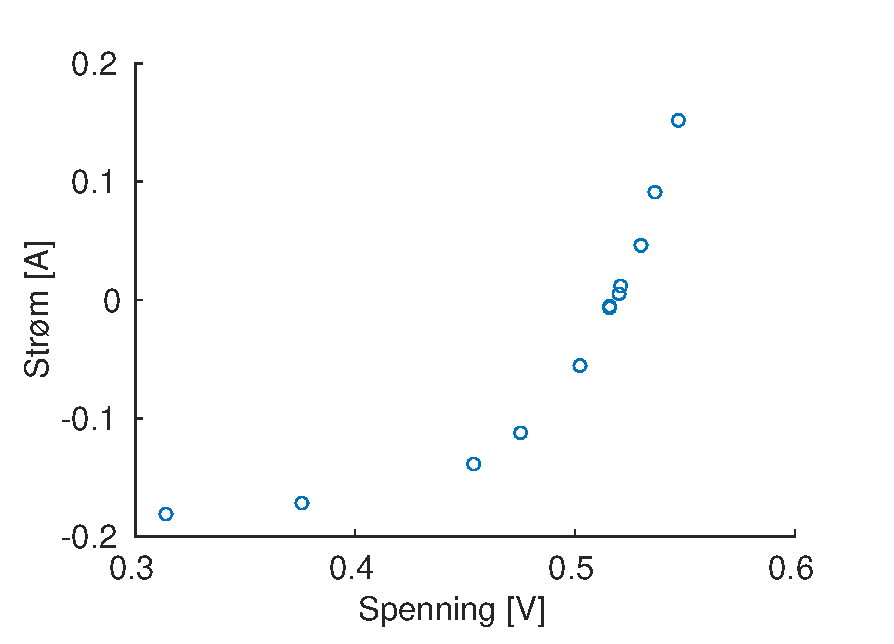
\includegraphics[width = 0.5\textwidth]{matlab/LAB/belystMedSpenning.eps}
	\caption{Strøm-spenning-karakteristikk for belyst solcelle med påtrykt spenning.}
	\label{fig:resMedSpenning}
\end{figure}

\subsubsection{Uten påtrykt spenning}
\begin{figure}[!ht]
	\includegraphics[width = 0.5\textwidth]{matlab/LAB/utenSpenning.eps}
	\caption{Strøm-spenning-karakteristikk for belyst solcelle med og uten påtrykt spenning.}
	\label{fig:resMedSpenning}
\end{figure}
\section{Diskusjon}

%\printbibliography
\clearpage
\onecolumn
\appendix


\section{Matlab-script}

\end{document}
